112. \begin{figure}[ht!]
\center{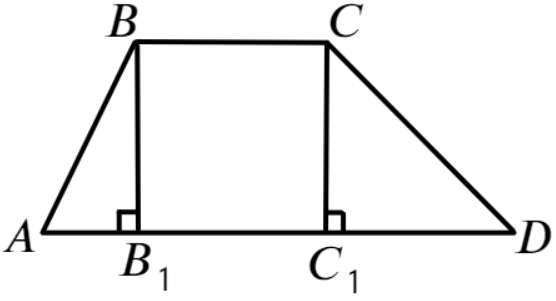
\includegraphics[scale=0.35]{g9-112.png}}
\end{figure}\\
Опустим высоты $BB_1$ и $CC_1.$ Пусть $AB_1=x,$ тогда $C_1D=9-5-x=4-x$ и $BB_1^2=4^2-x^2=CC_1^2=5^2-(4-x)^2,\ 16-x^2=25-16+8x-x^2,\ x=\cfrac{7}{8}.$ Тогда $BB_1=\sqrt{16-\cfrac{49}{64}}=\cfrac{5\sqrt{39}}{8}.$\\
